\documentclass[10pt,journal,compsoc]{IEEEtran}
\usepackage[utf8x]{inputenc} % caracteres latinos
\usepackage{graphicx} % inserção de figuras
\usepackage{amsmath,amssymb,bm} % entidades matemáticas
\usepackage{subcaption} % subfigures
\usepackage[nocompress]{cite} % referência bibliográfica

% bloco de código formatado
\usepackage{listings}
\usepackage{xcolor}
 
 % define cores como triplas (r,g,b) 0 < r,g,b < 1.
\definecolor{codegreen}{rgb}{0,0.6,0}
\definecolor{codegray}{rgb}{0.5,0.5,0.5}
\definecolor{codepurple}{rgb}{0.58,0,0.82}
\definecolor{backcolour}{rgb}{0.86,0.93,0.96}
 
\lstdefinestyle{mycode}{
    backgroundcolor=\color{backcolour},   
    commentstyle=\color{codegreen},
    keywordstyle=\color{magenta},
    numberstyle=\tiny\color{codegray},
    stringstyle=\color{codepurple},
    basicstyle=\ttfamily\footnotesize,
    breakatwhitespace=false,         
    breaklines=true,                 
    captionpos=b,                    
    keepspaces=true,                 
    numbers=left,                    
    numbersep=5pt,                  
    showspaces=false,                
    showstringspaces=false,
    showtabs=false,                  
    tabsize=2
}
 
\lstset{style=mycode}


% links no arquivo
\usepackage{hyperref}
\hypersetup{
    colorlinks=true,
    linkcolor=blue,
    filecolor=magenta,      
    urlcolor=cyan,
}
 
\urlstyle{same}

% efeito de papel rasgado 

\usepackage{framed}
\usepackage{tikz}
\usepackage[margin=1cm]{geometry}% for screen preview
\usetikzlibrary{decorations.pathmorphing,calc,shadows.blur,shadings}
\pgfmathsetseed{1} % To have predictable results
% Define a background layer, in which the parchment shape is drawn
\pgfdeclarelayer{background}
\pgfsetlayers{background,main}

% This is the base for the fractal decoration. It takes a random point between the start and end, and
% raises it a random amount, thus transforming a segment into two, connected at that raised point
% This decoration can be applied again to each one of the resulting segments and so on, in a similar
% way of a Koch snowflake.
\pgfdeclaredecoration{irregular fractal line}{init}
{
  \state{init}[width=\pgfdecoratedinputsegmentremainingdistance]
  {
    \pgfpathlineto{\pgfpoint{random*\pgfdecoratedinputsegmentremainingdistance}{(random*\pgfdecorationsegmentamplitude-0.02)*\pgfdecoratedinputsegmentremainingdistance}}
    \pgfpathlineto{\pgfpoint{\pgfdecoratedinputsegmentremainingdistance}{0pt}}
  }
}

% define some styles
\tikzset{
   paper/.style={draw=black!10, blur shadow,
                 lower left=black!20, upper left=black!15, upper right=white, lower right=black!10},
   irregular border/.style={decoration={irregular fractal line, amplitude=0.2},
           decorate,
     },
   ragged border/.style={ decoration={random steps, segment length=7mm, amplitude=2mm},
           decorate,
   }
}

% Macro to draw the shape behind the text, when it fits completly in the
% page
\def\tornpaper#1{
\tikz{
  \node[inner sep=1em] (A) {#1};  % Draw the text of the node
  \begin{pgfonlayer}{background}  % Draw the shape behind
  \fill[paper] % recursively decorate the bottom border
        decorate[irregular border]{decorate{decorate{decorate{decorate[ragged border]{
        ($(A.south east) - (0, random*5mm)$) -- ($(A.south west) - (0, random*5mm)$)
        }}}}}
        -- (A.north west) -- (A.north east) -- cycle;
  \end{pgfonlayer}}
} % inserindo arquivo externo de estilo

% correct bad hyphenation here
\hyphenation{Ma-te-ma-ti-ca-men-te}

\begin{document}

\title{Redes Neurais Artificiais \textit{for Dummies}: \\ 
       Praticando um pouco de \LaTeX{} no CI/UFPB}

\author{Gustavo~Oliveira,~\IEEEmembership{DCC/UFPB}
        e Rafael~Magalhães,~\IEEEmembership{DCX/UFPB}% <-this % stops a space
\IEEEcompsocitemizethanks{\IEEEcompsocthanksitem G.Oliveira \'{e} professor do 
Departamento de Computa\c{c}\~{a}o Cient\'{i}fica do Centro de Inform\'{a}tica 
da Universidade Federal da Para\'{i}ba.\protect\\
E-mail: gustavo.oliveira@ci.ufpb.br
\IEEEcompsocthanksitem G. Oliveira e R. Magalhães agradecem a sua aten\c{c}\~{a}o.}
\thanks{Manuscript received July 25, 2019; revised August 26, 2019.}}


\markboth{Journal of \LaTeX\ Class Files,~Vol.~14, No.~8, August~2015}%
{Oliveira \MakeLowercase{\textit{et al.}}: Bare Demo of IEEEtran.cls for Computer Society Journals}

\IEEEtitleabstractindextext{%
\begin{abstract}
Este artigo é um ensaio minimalista que tem o propósito de servir como texto-base para 
o mini-curso: \textit{Conhecendo o \LaTeX: usos, dicas e práticas}. Alguns tópicos 
sobre redes neurais artificiais são apresentados de maneira genérica. Com diversos 
elementos, mostramos como a linguagem \LaTeX é poderosa para manipular não apenas 
textos simples, mas também equações, figuras, tabelas, referências cruzadas e citações. 
Conclui-se que a ferramenta é muito eficaz para a produção de praticamente qualquer 
tipo de texto acadêmico.
\end{abstract}


\begin{IEEEkeywords}
Redes neurais artificiais, funções de ativação, Python, \LaTeX.
\end{IEEEkeywords}}

\maketitle

\IEEEdisplaynontitleabstractindextext
\IEEEpeerreviewmaketitle

% INTRODUÇÃO 
\IEEEraisesectionheading{\section{Introdução}\label{sec:introducao}}

\IEEEPARstart{O} cérebro humano contém em torno de 10\textsuperscript{11} neurônios. 
Cada um deles processa informações e se conecta com 
outros milhares de neurônios continuamente ou de modo 
paralelo. A estrutura individual de suas conexões e 
o comportamento conjunto destes nós naturias formam 
a base para o estudo das \textit{redes neurais artificiais} - RNAs.
A Figura \ref{fig:neuronio} contém uma ilustração simplificada
para um neurônio biológico. bem como seu modelo associado. 
Este modelo de neurônio artificial foi proposto por 
McCulloch e Pitts \cite{mcculloch1943logical} em 1943 e 
ficou conhecido como MCP.
\begin{figure}[h!]
  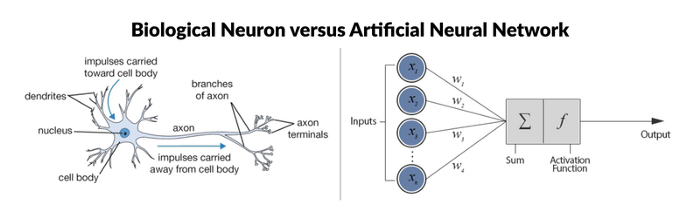
\includegraphics[scale=0.35]{figs/1mcp.png}
  \caption{Esquema de neurônio biológico e modelo MCP de 
  McCulloch e Pitts.}
  \label{fig:neuronio}
\end{figure}

\subsection{Aprendizagem: o perceptron}

RNAs possuem a capacidade de aprender por exemplos e tomar 
decisões sobre aquilo que aprendem. Para tanto, necessitam 
de um conjunto de procedimentos bem definidos que adaptam 
seus parâmetros, ou seja, um \textbf{algoritmo de aprendizagem}. 
Dessa maneira, define-se que

\begin{quotation}
aprendizagem é o processo pelo qual os parâmetros de uma rede
neural são ajustados através de uma forma continuada de estímulo
pelo ambiente no qual a rede está operando, sendo o tipo específico 
de aprendizagem realizada definido pela maneira particular 
como ocorrem os ajustes realizados nos parâmetros.
\end{quotation}

Desde a década de 1940, muito se aperfeiçoou na compreensão 
das redes artificiais. Em 1958, Frank Rosenblatt introduziu 
um novo modelo para o neurônio biológico formado por duas
unidades básicas: os \emph{nós} MCP e uma regra de aprendizado.
Este modelo foi denominado \texttt{perceptron}, o qual é utilizado
até hoje. Então, de meados da década de 1970 para cá, grande
progresso foi atingido com aprendizagem de máquina. 
Vejamos, por exemplo, a linha do tempo mostrada na 
Figura \ref{fig:historico}. 
\begin{figure*}[t!]
  \centering
  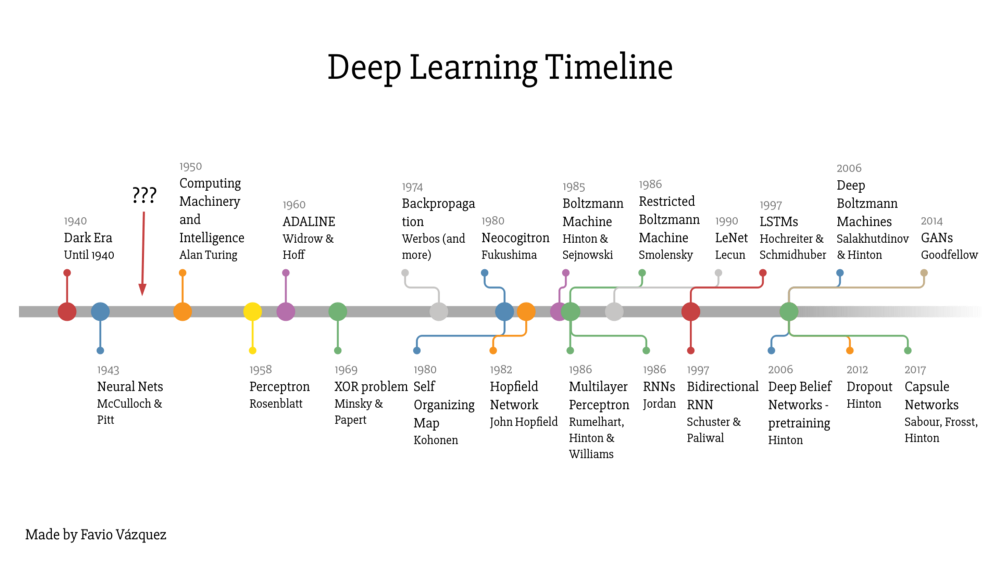
\includegraphics[scale=0.4,trim={1cm 3cm 1cm 5cm},clip]{figs/2timeline.png}
  \caption{Linha do tempo: \textit{deep learning}.}
  \label{fig:historico}
\end{figure*}

\section{Métodos}
\label{sec:metodos}

\subsection{Limiar de excitação}

Um neurônio biológico dispara quando a soma dos impulsos que ele recebe 
ultrapassa seu limiar de excitação (\textit{threshold}) $\theta$. 
Matematicamente, podemos modelar um neurônio $k$ pelo seguinte par de equações: 
\begin{equation}
    v_k = b_k + \displaystyle \sum_{j=1}^m w_{kj} x_j 
\end{equation}
e
\begin{equation}
    y_k = \phi(v_k),
\end{equation}
em que
\begin{itemize}
    \item $x_1,x_2,\ldots,x_m$ são \textbf{sinais de entrada};
    \item $w_{k1},w_{k2},\ldots,w_{km}$ são \textbf{pesos sinápticos};
    \item $u_k$ é o \textbf{adicionador} ou \textbf{combinador linear}; 
    \item $b_k$ é o \textbf{bias}\footnote{O \textit{bias} é um parâmetro externo 
    de entrada $x_0$ e peso $w_{k0} = b_k$ que tem o efeito de aumentar (se positivo) 
    ou diminuir (se negativo) a entrada líquida da função de ativação.};
    \item $v_k$ é o \textbf{potencial de ativação};
    \item $\phi$ é a \textbf{função de ativação};
    \item $y_k$ é a \textbf{saída}.
\end{itemize}
Quando $v_k > \theta$, o neurônio é ativado e produz uma saída. No caso do nó MCP, $y_k \in \{0,1\}$. 

\subsection{Funções de ativação}

Uma função de ativação define a saída do nó. A mais básica é a Heaviside, 
também conhecida como \textit{função de limiar}, definida na Eq. \eqref{eq:heaviside}.
\begin{equation}
\label{eq:heaviside}
\phi(v_k) = 
\begin{cases}
1, & \text{se} \, v_k \geq 0 \\
0, & \text{se} \, v_k < 0.
\end{cases}
\end{equation}

Outras funções de ativação são também utilizadas. A seguir, veremos mais dois exemplos.

\subsubsection{Função Relu}

A função Relu (\textit{rectified linear unit}) é definida como  
\begin{equation*} % sem referência.
\phi(v_k) = \max\{ 0, v_k \}.
\end{equation*}

\subsubsection{Função sigmoide}

A função sigmoide é definida como  
\begin{equation*} % sem referência.
\phi(v_k) = \frac{1}{1 + \exp(-a v_k)},
\end{equation*}
onde $a$ é um parâmetro de suavização.


\section{Resultados}
\label{sec:resultados}

\subsection{Códigos}
\label{subsec:codigos}

Podemos incluir um bloco de código que mostra como gerar 
gráficos em Python para as funções de ativação anteriores.

% 1. incluir versão pura
% 2. criar style.tex
% 3. importar style.tex
% 4. adicionar versão melhor
\lstinputlisting[language=Python,style=mycode,caption=Código Python.]{./py/func-ativ.py}

\subsection{Plotagens}

O código incluído na Subseção \ref{subsec:codigos} gera os gráficos mostrados
na Figura \ref{fig:plots}.
\begin{figure}
     \centering
     \begin{subfigure}[b]{0.3\textwidth}
         \centering
         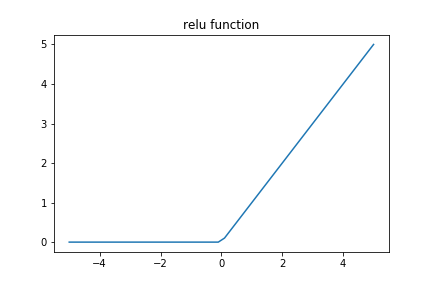
\includegraphics[width=\textwidth]{figs/relu.png}
         \caption{Relu.}
     \end{subfigure}
     \hfill
     \begin{subfigure}[b]{0.3\textwidth}
         \centering
         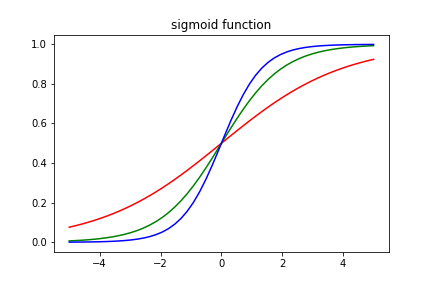
\includegraphics[width=\textwidth]{figs/sigmoid.png}
         \caption{Sig. { \color{red} ––} $a=0.5$
                            { \color{green} ––} $a=1$ 
                            { \color{blue} ––} $a=1.5$.
                 }
     \end{subfigure}
        \caption{Exemplos de funções de ativação.}
        \label{fig:plots}
\end{figure}

% bloco fantasia
\tornpaper{
\parbox{.7\columnwidth}
    {
        \LARGE{RNA!} \textit{\hspace{1cm}} \textbf{\Large{RNA!}} \\
        \medskip
        ~~~~ \small{RNA!} \\ 
        \qquad \qquad  \scriptsize{RNA!}
        \huge{\color{white}\textsc{RNA!}} \\
        \bigskip
        \large{RNA!} \, \! \ \ \ \ \Large{\color{blue}RNA!}
    }
}

\fbox{\parbox{3cm}\Huge{\textbf{RNA!}}} \\
\vspace{1cm}
\begin{center}
\fbox{\fbox{\fbox{\parbox{3cm}\Huge{\textbf{RNA!}}}}}
\end{center}

\section{Conclusão}

Neste texto, fizemos uma breve apresentação sobre o conceito de redes 
neurais artificiais. Introduzimos na seção \ref{sec:introducao}. 
Incluímos uma metodologia na \ref{sec:metodos} e resultados na 
seção \ref{sec:resultados}. Estudos têm avançado para muitos campos. Para encerrar,
incluímos um resumo sobre tipos de arquiteturas de RNAs na Tabela \ref{tab:resumo}.
% usar o latextablegenerator
% resizebox
\renewcommand{\arraystretch}{2.0}
\begin{table}[h!]
\resizebox{\columnwidth}{!}{
\begin{tabular}{ccc}
\textbf{no. de camadas} & \textbf{conexão nodal}    & \textbf{conectividade}  \\ \hline
única                   & feedforward (ou acíclica) & fracamente conectada    \\
múltiplas               & feedback (ou cíclica)     & completamente conectada
\end{tabular}
}
\caption{\label{tab:resumo}Tabela-resumo dos tipos de arquitetura de RNAs.}
\end{table}

Saiba mais sobre RNAs em \cite{haykin1994neural}, \cite{braga2007} e \cite{kovacs2002redes}.


\appendices

\section{Algumas equações para praticar a escrita}

Vide arquivo \texttt{desafio.tex}...

\section{Personalidades no estudo de RNAs}

\begin{enumerate}
    \item Warren S. McCulloch ($\star$ 1868 - $\dagger$ 1969) \\ 
    \item Walter Pitts ($\star$ 1923 - $\dagger$ 1969) \\ 
    \item Frank Rosenblatt ($\star$ 1928 - $\dagger$ 1971) \\ 
\end{enumerate}
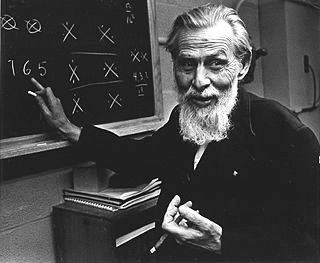
\includegraphics[scale=0.37]{figs/a-1mcculloch.jpeg}
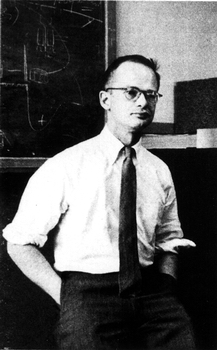
\includegraphics[scale=0.278]{figs/a-2pitts.jpg}
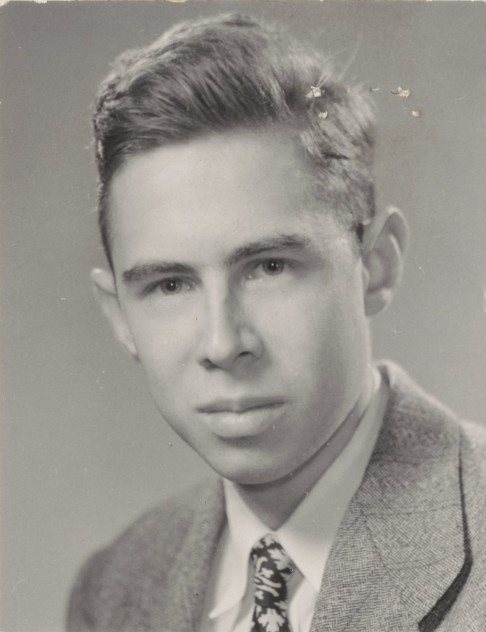
\includegraphics[scale=0.154]{figs/a-3rosenblatt.jpeg}


% use section* for acknowledgment
\ifCLASSOPTIONcompsoc
  % The Computer Society usually uses the plural form
  \section*{Acknowledgments}
\else
  % regular IEEE prefers the singular form
  \section*{Acknowledgment}
\fi
G.O. agradece a oportunidade de ministrar este mini-curso.


% bibliografia
\bibliographystyle{IEEEtran}
\bibliography{IEEEabrv,refs}


% biografia
%\begin{IEEEbiography}[{\includegraphics[width=1in,height=1.25in,clip,keepaspectratio]{figs/gustavo}}]{Gustavo Oliveira}
\begin{IEEEbiographynophoto}{Gustavo Oliveira}
Prof. do DCC/CI/UFPB e pesquisador do LaMEP. \\
Visite-nos em: \url{lamep.ci.ufpb.br}.
\end{IEEEbiographynophoto}

\begin{IEEEbiographynophoto}{Rafael Magalhães}
Prof. do DCX/CCAE/UFPB e pesquisador no LaMEP/UFPB.
\end{IEEEbiographynophoto}

\end{document}
